\documentclass{beamer}
\usetheme{CambridgeUS}
\usecolortheme{dolphin}
\title[Generative models for shape parametrization]{Generative models for shape parametrization}
\author[G. Padula]{\textbf{Guglielmo Padula}}
\institute{University of Trieste}

\date{}

\usepackage{graphicx}

\begin{document}
\begin{frame}{Bonus: measures of simulation}
As I said before, we can run simulation on the sample mesh, calculate some measures of interest, and then comparing the distributions. 
\begin{itemize}
\item Drag coefficient $C_{D}$ 
\item L2 of Drag force $||F_D||_{2}^{2}=||\frac{1}{2} \rho v^2 C_D A||_{2}^{2}$
\item Momentum $mv_{x}$
\end{itemize}
\end{frame}

\begin{frame}{Bonus: Drag Coefficient}
\makebox[\textwidth]{%
\begin{minipage}{1.00\textwidth} % <--- can be as large the slide size permits
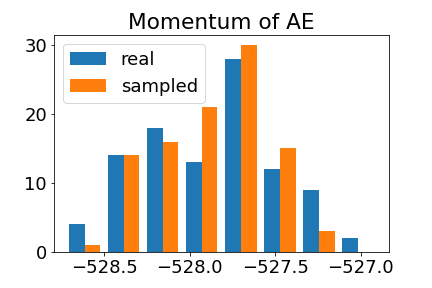
\includegraphics[width=.47\textwidth,keepaspectratio]{dragAE}\hfill%
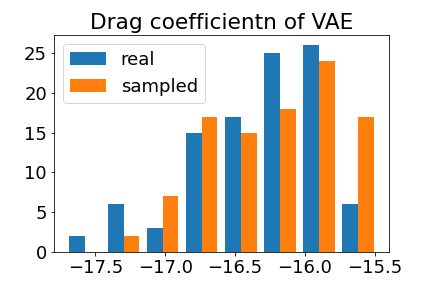
\includegraphics[width=.47\textwidth,keepaspectratio]{dragVAE}\\[0.001pt]
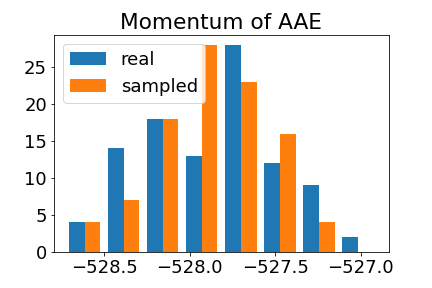
\includegraphics[width=.47\textwidth,keepaspectratio]{dragAAE}\hfill%
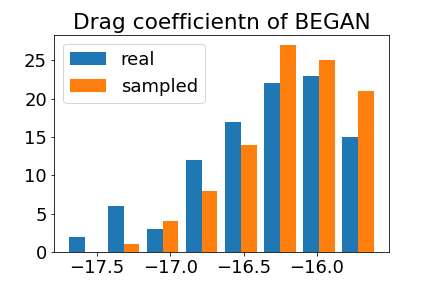
\includegraphics[width=.47\textwidth,keepaspectratio]{dragBEGAN}
\end{minipage}
}
\end{frame}
\begin{frame}{Bonus: L2 Coefficient}
\makebox[\textwidth]{%
\begin{minipage}{1.00\textwidth} % <--- can be as large the slide size permits
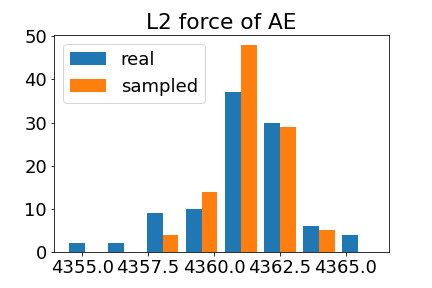
\includegraphics[width=.47\textwidth,keepaspectratio]{L2AE}\hfill%
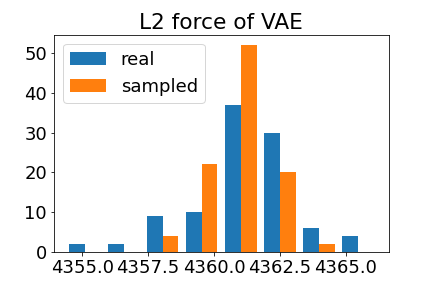
\includegraphics[width=.47\textwidth,keepaspectratio]{L2VAE}\\[0.001pt]
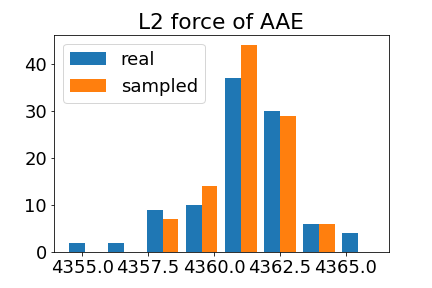
\includegraphics[width=.47\textwidth,keepaspectratio]{L2AAE}\hfill%
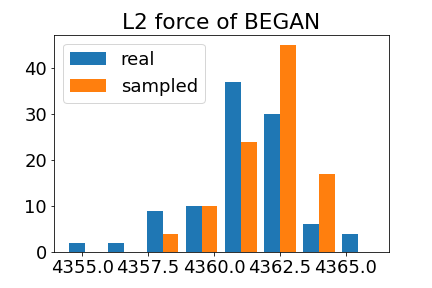
\includegraphics[width=.47\textwidth,keepaspectratio]{L2BEGAN}
\end{minipage}
}
\end{frame}
\begin{frame}{Bonus: Momentum Coefficient}
\makebox[\textwidth]{%
\begin{minipage}{1.00\textwidth} % <--- can be as large the slide size permits
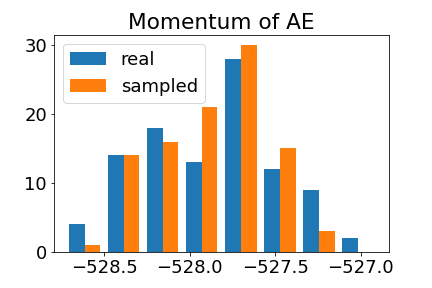
\includegraphics[width=.47\textwidth,keepaspectratio]{momAE}\hfill%
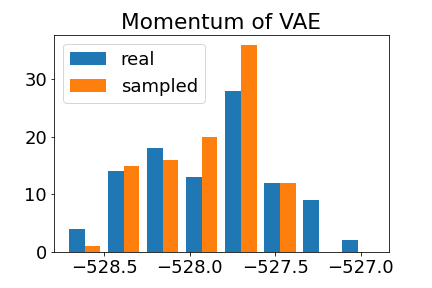
\includegraphics[width=.47\textwidth,keepaspectratio]{momVAE}\\[0.001pt]
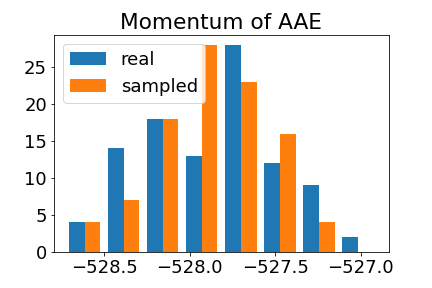
\includegraphics[width=.47\textwidth,keepaspectratio]{momAAE}\hfill%
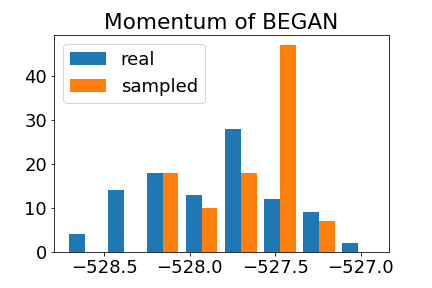
\includegraphics[width=.47\textwidth,keepaspectratio]{momBEGAN}
\end{minipage}
}
\end{frame}
\begin{frame}{Results}
\begin{table}[H]
\begin{tabular}{|l|l|l|l|l|}
\hline
&   AE & AAE &  VAE &  BEGAN  \\ \hline
$RelMMD(Drag)$ & 0.04 & 0.05 &  0.05 &  0.06 \\ \hline
$RelMMD(Momentum)$  &  0.04 &  0.05 & 0.06 &  0.14  \\ \hline
$RelMMD(L2)$ & 0.12 & 0.13 &  0.16	 &  0.24 \\ \hline
\end{tabular}
\end{table}
\end{frame}
\end{document}